\section{Mathematical Methodology and Index Formulation}
\label{sec:methodology}

\subsection{Pan-India Baseline Normalization}
To preserve true seasonal climate cycles and cross-city comparability without falling into the seasonal normalization trap, all five physical drivers are standardized against a single, frozen empirical baseline fitted on the comprehensive pan-India panel ($N = 334,332$) across all seven metropolitan regions and 36 observation months:
\begin{equation}
    S_{j, i, t} = \text{clip}\left(\frac{x_{j, i, t} - q_{0.02}(X_{j})}{q_{0.98}(X_{j}) - q_{0.02}(X_{j})}, 0.0, 1.0\right)
\end{equation}
where $x_{j, i, t}$ is the native physical driver $j$ in hexagonal cell $i$ at month $t$; $q_{0.02}$ and $q_{0.98}$ are the 2nd and 98th empirical percentiles of driver $j$ evaluated across all 334,332 observations. Clamping extreme outliers at the 2nd and 98th quantiles shields the operational scale from rogue sensor spikes while strictly guaranteeing that all standardized sub-indices:
\begin{equation}
    S_{\text{heat}}, \ S_{\text{water}}, \ S_{\text{veg}}, \ S_{\text{pollution}}, \ S_{\text{exposure}} \in [0.0, 1.0]
\end{equation}
are non-negative, dimensionless, and positively oriented toward higher stress.

\begin{figure}[t]
    \centering
    \IfFileExists{figures/Figure2_inter_indicator_correlation.png}{%
        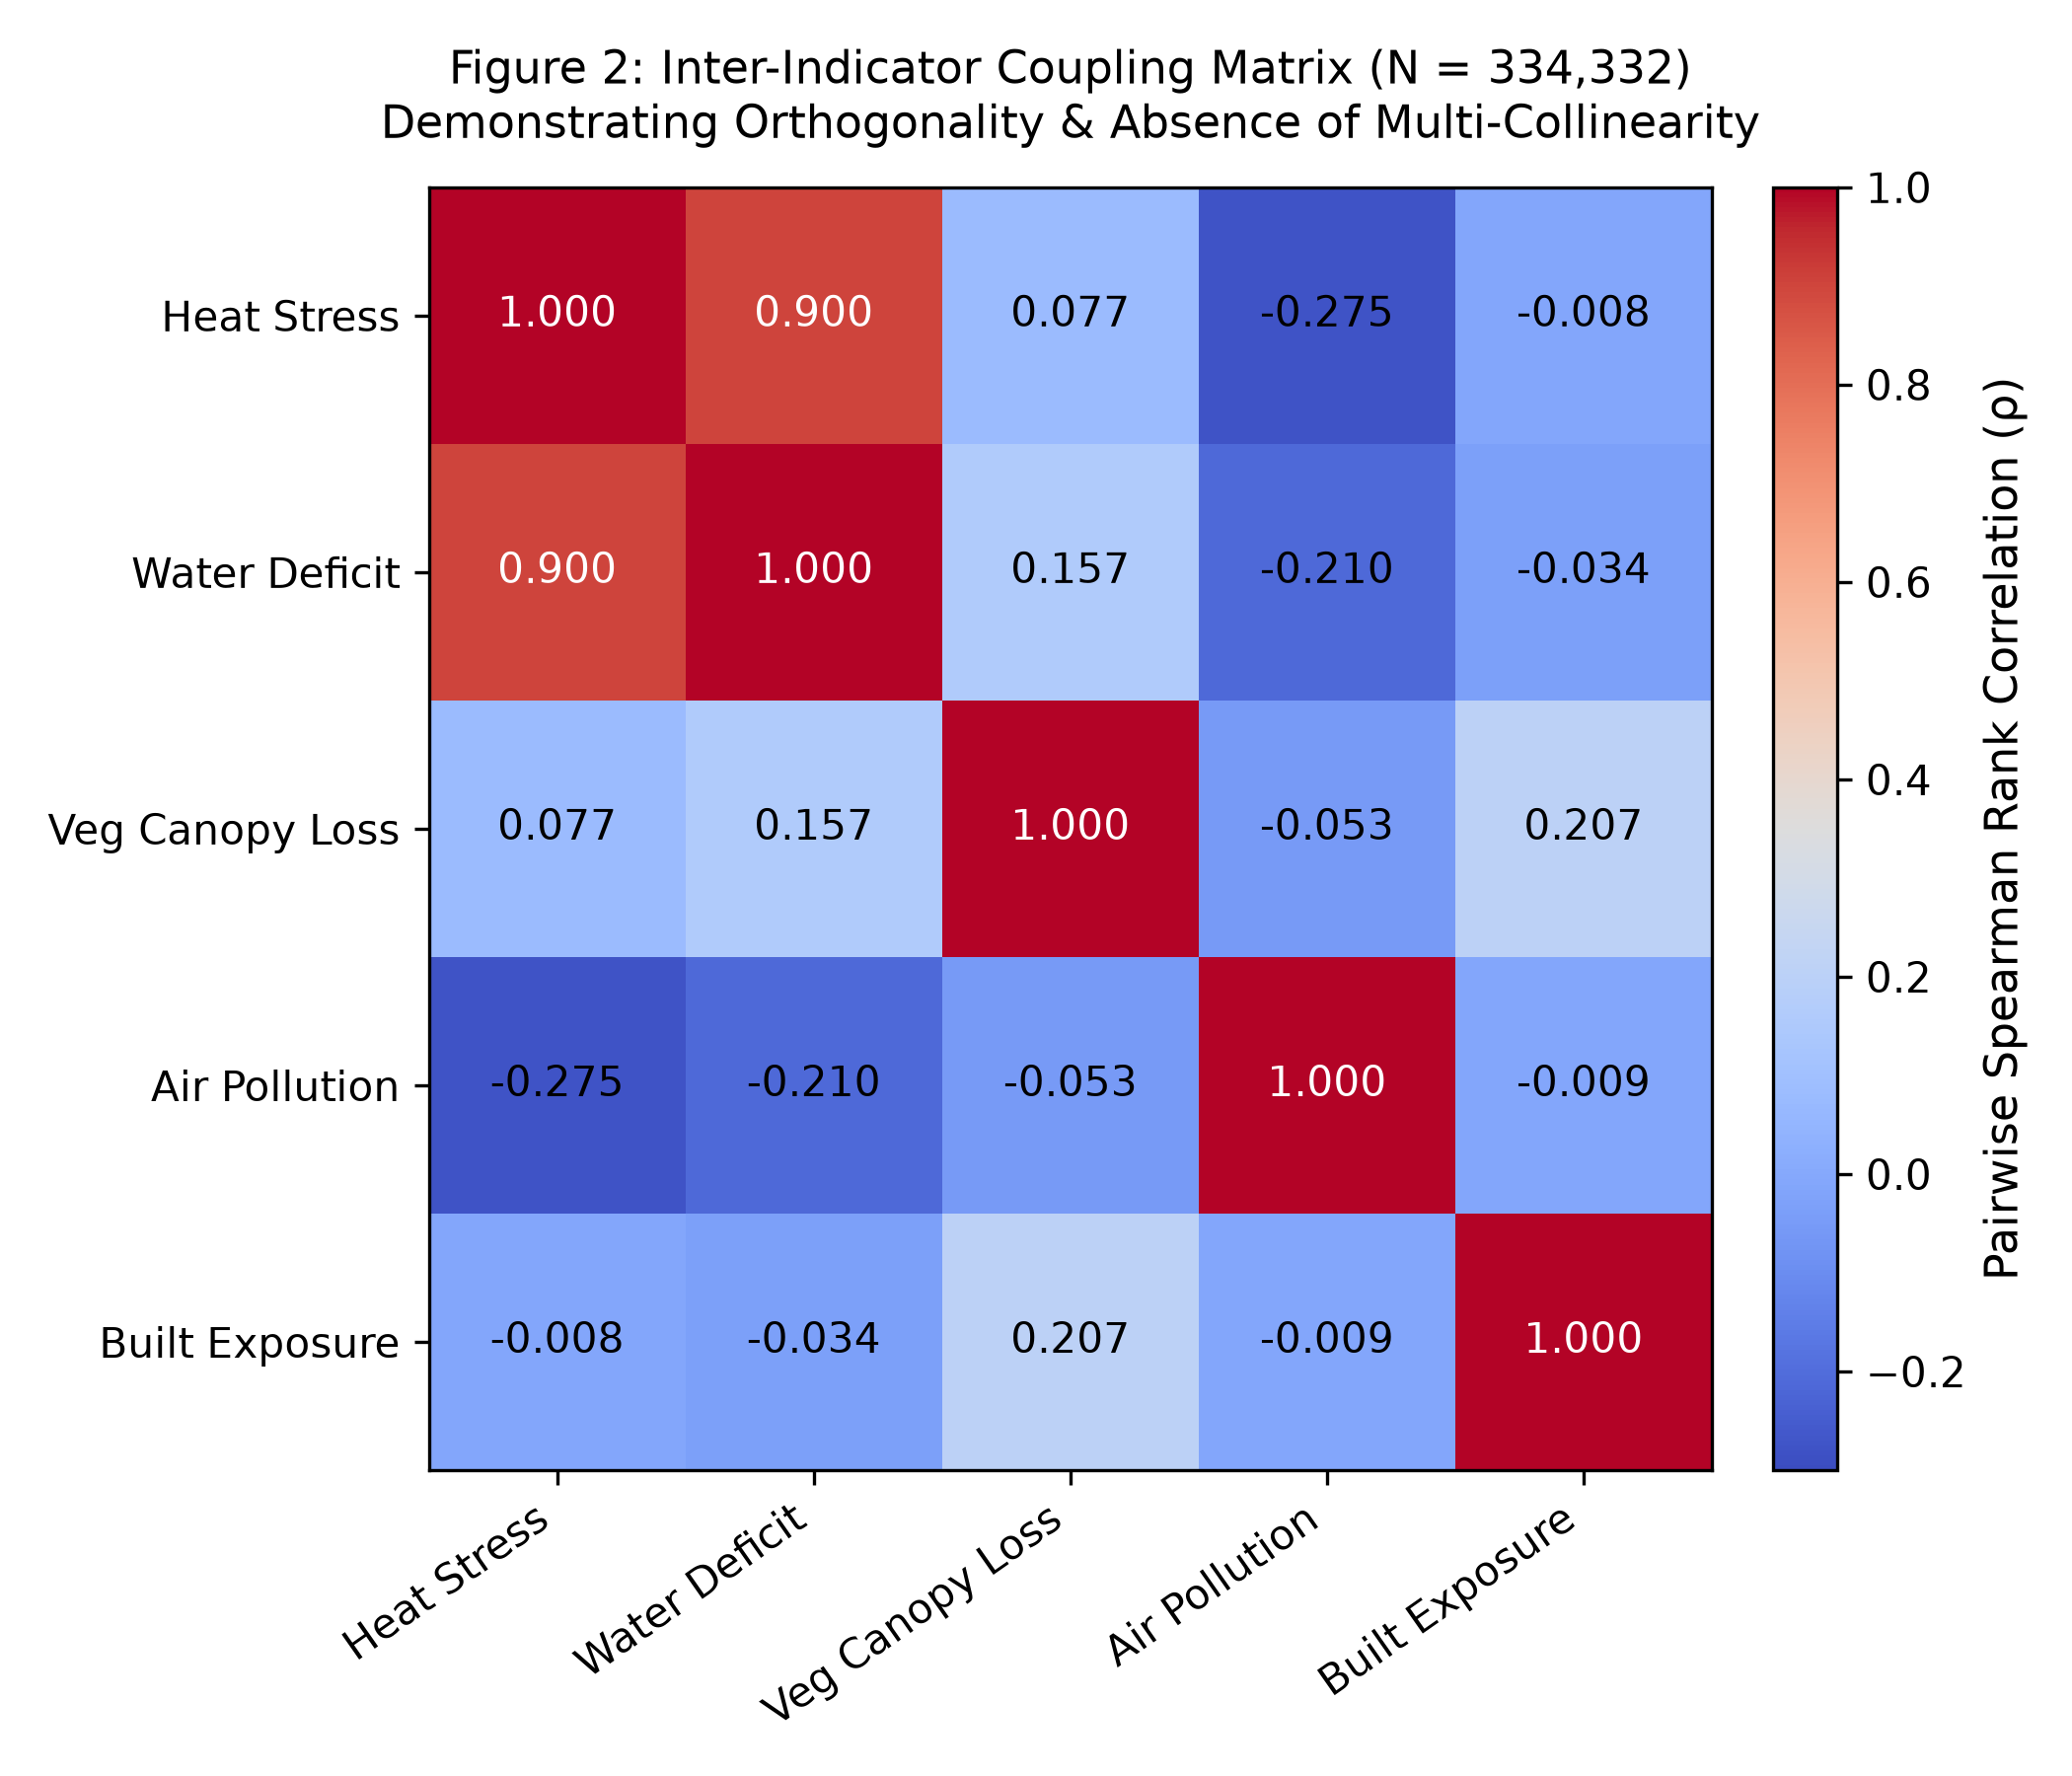
\includegraphics[width=0.7\textwidth]{figures/Figure2_inter_indicator_correlation.png}%
    }{%
        \vspace{1em}
        \fbox{\parbox{0.75\textwidth}{\centering\small\textbf{[Figure 2: Inter-Indicator Orthogonality Heatmap]}\\
        \textit{Generated via \texttt{colab\_analysis.py} from \texttt{final\_7\_cities.parquet} ($N = 334,332$). Demonstrates absence of harmful collinearity ($\text{VIF} < 1.12$, max pairwise $\rho = 0.303$).}}}%
        \vspace{1em}
    }
    \caption{Pairwise Spearman rank correlation matrix across the five standardized environmental stress dimensions evaluated across all $N = 334,332$ panel records. Low inter-indicator correlations confirm domain orthogonality and prevent multi-collinearity inflation.}
    \label{fig:correlation_matrix}
\end{figure}

\subsection{Linear Base Weighting Philosophies}
The linear composite baseline ($\text{SSI}_{\text{lin}}$) represents the multi-dimensional weighted sum across the five standardized environmental stress dimensions:
\begin{equation}
    \text{SSI}_{\text{lin}, i, t} = \sum_{j=1}^{5} w_j \cdot S_{j, i, t}, \quad \text{subject to} \quad \sum_{j=1}^{5} w_j = 1, \quad w_j \ge 0
\end{equation}
To ensure methodological defensibility and test parametric sensitivity, we evaluate four candidate weighting schemes fitted across all 334,332 observations (Table~\ref{tab:weights_comparison} and Figure~\ref{fig:weighting_schemes}):

\begin{table}[t]
\centering
\small
\caption{Comparison of indicator weights derived across the four candidate weighting schemes fitted on the pan-India multi-biome panel ($N = 334,332$ observations across all seven metropolitan regions).}
\label{tab:weights_comparison}
\begin{tabularx}{\textwidth}{@{}X r r r r@{}}
\toprule
\textbf{Indicator Dimension} & \textbf{Equal ($w_{\text{eq}}$)} & \textbf{Entropy ($w_{\text{ewm}}$)} & \textbf{CRITIC ($w_{\text{cr}}$)} & \textbf{PCA ($w_{\text{pca}}$)} \\
\midrule
Heat Stress ($S_{\text{heat}}$) & \textbf{0.2000} & 0.2989 & 0.2105 & 0.3586 \\
Climatic Water Deficit ($S_{\text{water}}$) & \textbf{0.2000} & 0.2188 & 0.2008 & 0.3614 \\
Vegetation Canopy Loss ($S_{\text{veg}}$) & \textbf{0.2000} & 0.0473 & 0.1265 & 0.1094 \\
Particulate Air Pollution ($S_{\text{pollution}}$) & \textbf{0.2000} & 0.1565 & 0.2687 & 0.1517 \\
Physical Built Exposure ($S_{\text{exposure}}$) & \textbf{0.2000} & 0.2785 & 0.1935 & 0.0189 \\
\midrule
\textbf{Sum} & \textbf{1.0000} & \textbf{1.0000} & \textbf{1.0000} & \textbf{1.0000} \\
\midrule
PC1 Variance Explained & --- & --- & --- & 40.18\% \\
Rank Correlation vs.\ Equal ($\rho$) & Baseline & 0.9691 & 0.9857 & 0.8919 \\
\bottomrule
\end{tabularx}
\end{table}


\begin{figure}[t]
    \centering
    \IfFileExists{figures/Figure4_weighting_schemes.png}{%
        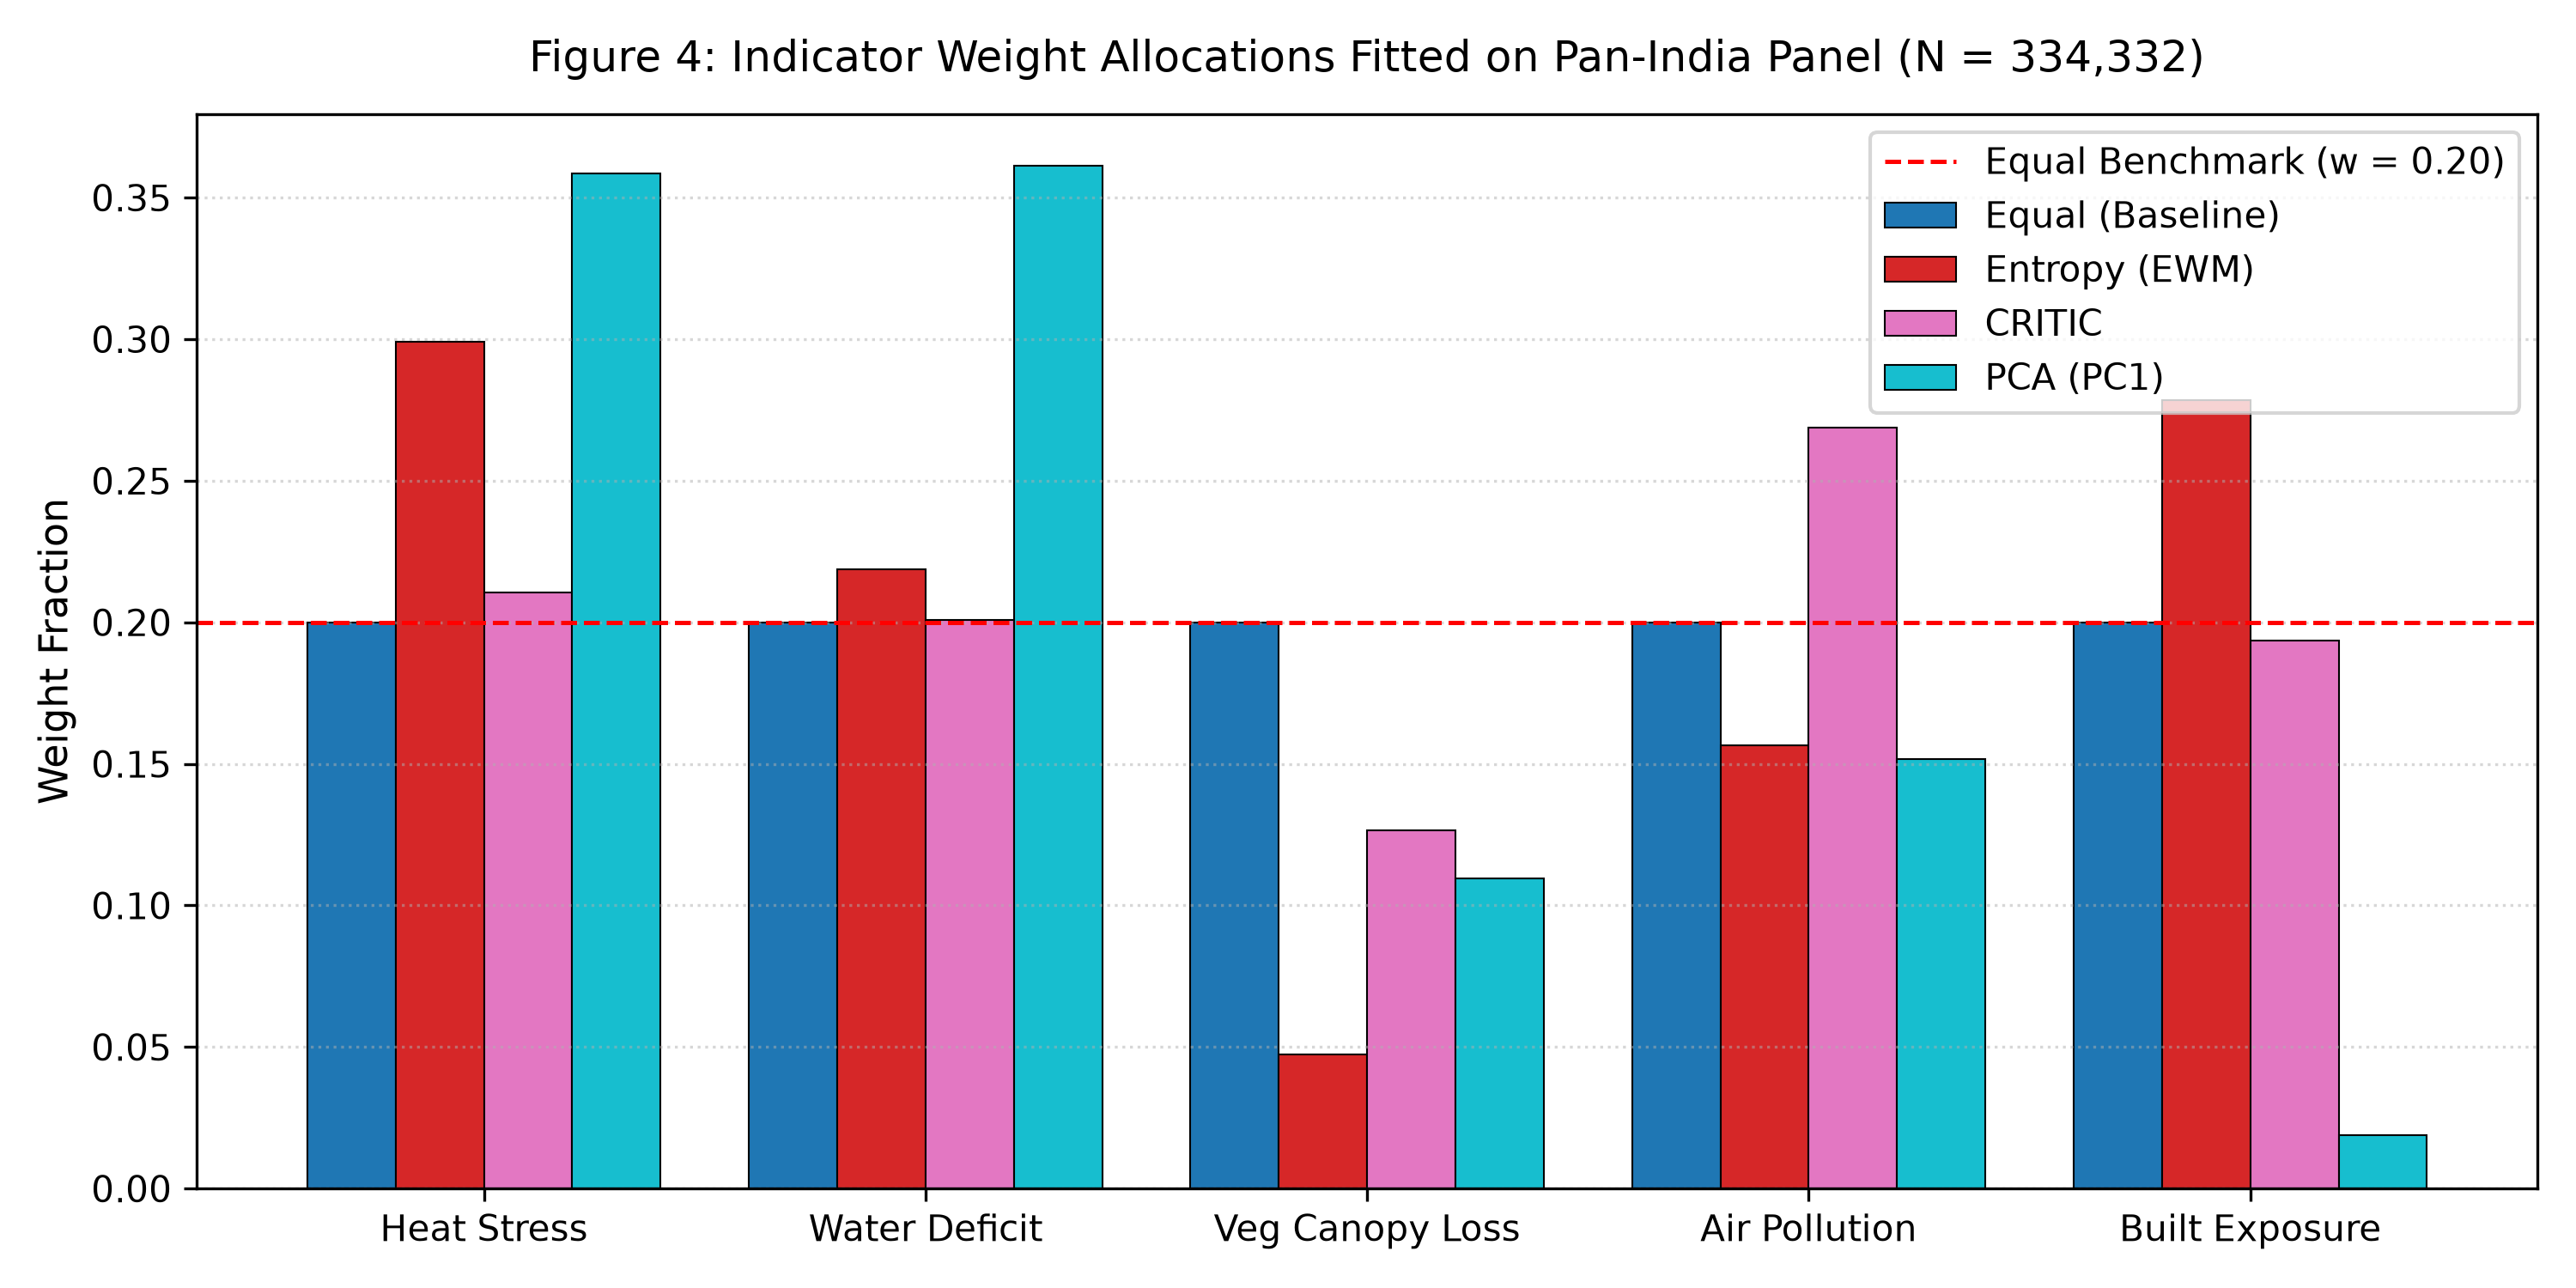
\includegraphics[width=0.85\textwidth]{figures/Figure4_weighting_schemes.png}%
    }{%
        \vspace{1em}
        \fbox{\parbox{0.85\textwidth}{\centering\small\textbf{[Figure 4: Indicator Weight Allocations Across Schemes]}\\
        \textit{Generated via \texttt{colab\_analysis.py} from \texttt{final\_7\_cities.parquet} ($N = 334,332$). Compares Equal, EWM, CRITIC, and PCA weight allocations.}}}%
        \vspace{1em}
    }
    \caption{Empirical weight allocations for the five sustainability dimensions derived across the full multi-biome panel ($N = 334,332$). While Entropy (EWM) and CRITIC balance contrast and conflict, PCA collapses built exposure ($w = 0.0189$), supporting equal weighting as the primary normative baseline.}
    \label{fig:weighting_schemes}
\end{figure}

\begin{enumerate}
    \item \textbf{Equal Weighting ($w_{\text{equal}}$ -- Primary Baseline):} 
    \begin{equation}
        w_j = \frac{1}{M} = 0.2000 \quad (\forall j \in \{1, \dots, 5\})
    \end{equation}
    Under the OECD Guidelines on Composite Indicators \citep{oecd2008handbook}, equal weighting represents the standard normative baseline when indicators measure distinct, non-substitutable environmental hazard domains without empirically calibrated damage functions. It prevents temporal weather swings from arbitrarily penalizing stationary physical infrastructure.
    
    \item \textbf{Entropy Weight Method ($w_{\text{ewm}}$):} Quantifies intrinsic information dispersion through Shannon entropy \citep{shannon1948mathematical}:
    \begin{equation}
        P_{ij} = \frac{S_{ij} + \epsilon}{\sum_{i=1}^{n} (S_{ij} + \epsilon)}, \quad e_j = -\frac{1}{\ln n}\sum_{i=1}^{n} P_{ij} \ln P_{ij}, \quad w_j = \frac{1 - e_j}{\sum_{k=1}^{M} (1 - e_k)}
    \end{equation}
    Higher weight is assigned to variables exhibiting greater spatial-temporal contrast across the observation matrix ($w_{\text{heat}} = 0.2989$, $w_{\text{exposure}} = 0.2785$).
    
    \item \textbf{CRITIC Method ($w_{\text{critic}}$):} Synthesizes contrast intensity (standard deviation $\sigma_j$) with inter-criteria correlation conflict \citep{diakoulaki1995determining}:
    \begin{equation}
        C_j = \sigma_j \sum_{k=1}^{M} (1 - r_{jk}), \quad w_j = \frac{C_j}{\sum_{k=1}^{M} C_k}
    \end{equation}
    where $r_{jk}$ is the pairwise Pearson correlation between sub-indices $j$ and $k$.
    
    \item \textbf{Principal Component Analysis ($w_{\text{pca}}$):} Derived from the normalized absolute eigenvector loadings of the first principal component ($V_1$) via Singular Value Decomposition:
    \begin{equation}
        w_j = \frac{|V_{1j}|}{\sum_{k=1}^{M} |V_{1k}|}
    \end{equation}
    Across all seven biomes, PC1 accounts for $40.18\%$ of nationwide variance, assigning $0.3614$ to water deficit and $0.3586$ to heat stress, but collapsing built exposure to $0.0189$.
\end{enumerate}

\subsection{Smooth Asymptotic Non-Linear Compound Coupling}
In accordance with IPCC AR6 frameworks on compound hazard interactions \citep{zscheischler2018future}, acute environmental stress escalates non-linearly when multiple stressors simultaneously breach critical threshold limits.

First, we define a bivariate joint-tail compound activation indicator ($\Omega_{\text{compound}} \in \{0, 1\}$) for the primary heat--air pollution hazard pair:
\begin{equation}
    \Omega_{\text{compound}, i, t} = \mathbb{I}\left(S_{\text{heat}, i, t} \ge q_{0.90}(S_{\text{heat}})\right) \times \mathbb{I}\left(S_{\text{pollution}, i, t} \ge q_{0.90}(S_{\text{pollution}})\right)
\end{equation}
where $\mathbb{I}(\cdot)$ is the Heaviside indicator function, and $q_{0.90}$ represents the 90th percentile threshold evaluated on the pan-India panel.

To overcome the ceiling clipping distortions of naive additive formulations, we formulate a \textbf{smooth asymptotic coupling equation}:
\begin{equation}
    \label{eq:smooth_ssi}
    \text{SSI}_{i, t} = \text{SSI}_{\text{lin}, i, t} + \gamma \cdot \Omega_{\text{compound}, i, t} \cdot \left(1.0 - \text{SSI}_{\text{lin}, i, t}\right)
\end{equation}
where $\gamma = 0.30$ represents the empirical coupling intensity parameter. 

The term $(1.0 - \text{SSI}_{\text{lin}})$ acts as an endogenous mathematical damping factor: as baseline linear stress approaches unity, the incremental compound amplification gracefully decelerates toward zero. This guarantees that:
\begin{equation}
    0.0 \le \text{SSI} \le 1.0 \quad \text{strictly without hard boundary truncation artifacts.}
\end{equation}

\subsection{Categorical Risk Banding}
To assist municipal stakeholders with prioritized resource allocation, continuous SSI scores are translated into four standardized categorical risk bands using pan-India quartile cuts:
\begin{equation}
    \text{Risk Band} = \begin{cases}
        \text{Low}, & \text{SSI} \le c_1 \quad (c_1 = 0.3284) \\
        \text{Moderate}, & c_1 < \text{SSI} \le c_2 \quad (c_2 = 0.4616) \\
        \text{High}, & c_2 < \text{SSI} \le c_3 \quad (c_3 = 0.6570) \\
        \text{Extreme}, & \text{SSI} > c_3
    \end{cases}
\end{equation}

\subsection{Spatial Block Bootstrapping for Autocorrelation Control}
Contiguous hexagonal micro-cells display substantial spatial autocorrelation, which invalidates classical independent and identically distributed (i.i.d.) variance estimators. To construct uninflated confidence intervals for all empirical metrics, we implement a \textbf{Spatial Block Bootstrap protocol}:
\begin{itemize}
    \item \textbf{Spatial Block Definition:} Cells are clustered into their Uber H3 Resolution~6 parent blocks ($\sim 36\text{ km}^2$, parent offset = 2).
    \item \textbf{Block Resampling:} Entire geographic parent clusters are sampled with replacement ($B = 500$ bootstrap iterations).
    \item \textbf{Confidence Intervals:} Empirical 95\% confidence intervals ($[\text{CI}_{0.025}, \text{CI}_{0.975}]$) are computed directly from the empirical cluster bootstrap distribution.
\end{itemize}

\subsection{Unsupervised Stress Typology: Archetype Clustering}
To extract operational spatial profiles across India's urban fabric, stationary hexagonal features (mean SSI, seasonal amplitude, mean heat, mean vegetation, exposure, and compound trigger frequency) are standardized and classified via unsupervised $k$-means clustering \citep{macqueen1967some}. Optimal cluster partitions ($k \in [2, 8]$) are evaluated using the silhouette coefficient \citep{rousseeuw1987silhouettes} and 50-fold bootstrap Adjusted Rand Index (ARI) stability.
